\documentclass[9pt,a4paper,twocolumn,twoside]{rho-class/rho}

% --- 1. Idioma y matemáticas básicas ---
\usepackage[spanish,es-nodecimaldot,es-noindentfirst,es-noshorthands]{babel}


% --- 2. EL TRUCO DE MAGIA (BIEN ESCRITO) ---
% Borramos los comandos problemáticos usando su nombre exacto interno
\expandafter\let\csname not=\endcsname\relax
\expandafter\let\csname not<\endcsname\relax
\expandafter\let\csname not>\endcsname\relax

% Ahora ya podemos cargar la fuente moderna sin que explote
\usepackage{fontspec}
\usepackage{unicode-math}
% --- 3. Bibliografía ---
\addbibresource{rho.bib}

% --- 4. Datos del Informe ---
\title{Estudio de la carga del electrón en el experimento de Millikan}
\author{Edgar Fernández Vigil}
\affil{Física - Facultad de Ciencias - Universidad de Oviedo}
\dates{\today}
\journalname{TEIII - Práctica de Laboratorio}
\journal{Carga del electrón en el experimento de Millikan}

% --- 5. Resumen ---
\begin{abstract}
En este informe se presenta la determinación experimental de la carga elemental $e$ mediante el método de la gota de aceite de Millikan. %
El experimento se fundamenta en el estudio de la dinámica de pequeñas gotas de aceite atomizadas que, tras adquirir carga por fricción, se desplazan en el seno de un campo eléctrico uniforme generado por un condensador de placas. %
Mediante la medición de las velocidades terminales de ascenso y descenso (o suspensión), y considerando el balance entre las fuerzas gravitatoria, de empuje, eléctrica y de fricción viscosa, se calculó la carga total de diversas muestras. %
Para asegurar la precisión de los resultados, se aplicó la corrección de Cunningham a la ley de Stokes, necesaria debido al tamaño microscópico de las gotas en relación con el camino libre medio del aire. %
Finalmente, a través de un análisis estadístico de minimización, se obtuvo el valor de la carga elemental y su incertidumbre, contrastándolo con el valor de referencia de $1.602 \cdot 10^{-19}$ C para verificar la cuantización de la carga eléctrica. %
\end{abstract}
% ----------------------------------------------------------
\begin{document}

    \maketitle
    \thispagestyle{firststyle}

\section{Introducción}

\rhostart{E}ntre los años 1910 y 1913, Robert Andrews Millikan logró determinar el valor de la carga elemental con una exactitud hasta ese momento no alcanzada, demostrando así la cuantización de la carga eléctrica. % 
Por este logro obtuvo el premio Nobel de Física en 1923. % 
Su experimento se basa en la medición de la cantidad de carga de gotitas de aceite que ascienden en el aire dentro del campo eléctrico de un condensador de placas, y descienden cuando no hay campo eléctrico. % 
El valor que determinó en su momento, $e=(1.592\pm0.003)\cdot10^{-19}$ C, se desvía apenas un 0.6\% del valor aceptado en la actualidad. % 


El análisis teórico asume que la gotita tiene forma esférica y está sometida a varias fuerzas: la fuerza gravitatoria ($F_G$), el empuje ascensional en el aire ($F_A$), la fuerza del campo eléctrico ($F_E$) y la fuerza de fricción de Stokes ($F_{R1,2}$). % 
Del balance de estas fuerzas al ascender con campo y al descender sin él, se pueden extraer expresiones para el radio y la carga de la gotita en función de las velocidades de ascenso ($v_1$) y descenso ($v_2$) medidas. % 
Además, al tratarse de radios muy pequeños que están en el orden de magnitud del camino libre medio de las moléculas del aire, es necesario corregir empíricamente la fuerza de fricción de Stokes para asegurar la validez de los cálculos. % 
    \begin{figure}[H]
        \centering
        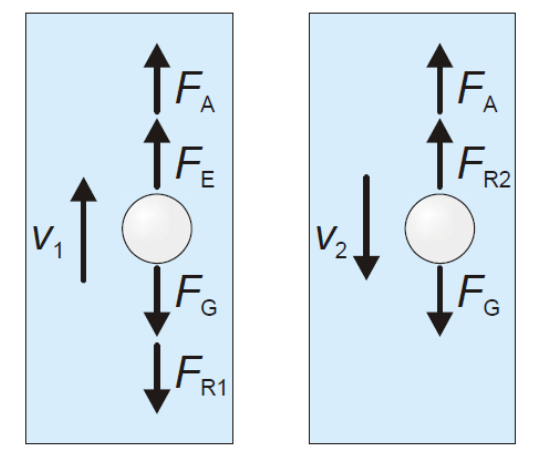
\includegraphics[width=0.7\columnwidth]{img/planteamiento-teorico-carga-elec.png}
        \caption{Planteamiento teórico del balance de fuerzas.}
        \label{fig:planteamiento-teorico-carga-elec}
    \end{figure}
\section{Objetivos}

La finalidad de esta práctica es: % 

\begin{itemize}
    \item Comprender experimentalmente la medida de la carga elemental mediante el experimento de Millikan. % 
    \item Realizar la medición de la velocidad de las gotas de aceite empleando dos técnicas distintas: el método de ascenso y el método de la suspensión. % 
    \item Aplicar las correcciones microscópicas a la fricción de Stokes para calcular con precisión el radio corregido ($r$) y la carga corregida ($q$) de cada gotita estudiada. % 
    \item Determinar el número entero de cargas elementales ($n$) presentes en cada gota mediante la minimización directa de la función de desviación $F(\hat{e})$. % 
    \item Obtener el valor experimental final de la carga elemental ($e$) y su respectiva incertidumbre realizando una media ponderada de las medidas, para finalmente compararlo con el valor de referencia. % 
\end{itemize}

\section{Dispositivo Experimental}

El montaje empleado consiste en una unidad compacta diseñada para el experimento de Millikan que integra los siguientes componentes: % 

\begin{itemize}
    \item \textbf{Cámara de experimentación:} Estructura desarmable que contiene un condensador de placas plano-paralelas con una separación de $d = 3$ mm. % 
    \item \textbf{Sistema de pulverización:} Pulverizador de aceite conectado a una bola de soplador para la introducción de microgotas en la celda. % 
    \item \textbf{Óptica de medición:} Microscopio equipado con un objetivo de aumento 2x y un ocular de 15x, que incluye una escala graduada de 10 mm con divisiones equivalentes a 50 $\mu$m reales en el plano de la muestra. % 
    \item \textbf{Unidad de control:} Generador de tensión regulable (0-600 V) con conmutador de polaridad, interruptores de cronometraje y pantalla para la visualización de parámetros. % 
    \item \textbf{Adquisición digital:} Cámara adaptada al microscopio que permite la visualización y grabación de las gotas en tiempo real mediante un PC. % 
\end{itemize}
    \begin{figure}[H]
        \centering
        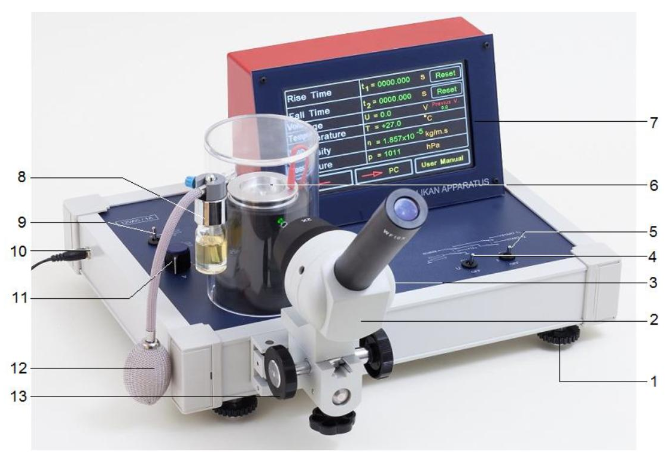
\includegraphics[width=0.7\columnwidth]{img/dispositivo-experimental-carga-elec.png}
        \caption{Esquema del dispositivo experimental.}
        \label{fig:Dispositivo}
    \end{figure}

\section{Procedimiento Experimental}

El procedimiento se basa en el seguimiento óptico de gotas de aceite mediante un microscopio de medición y una cámara acoplada a un ordenador para el registro de tiempos. % 
El desarrollo de la toma de datos se divide en las siguientes fases:

\subsection{Preparación y selección de la muestra}
Se introdujeron gotas de aceite en la cámara de experimentación mediante el pulverizador. % 
Utilizando la iluminación LED y el microscopio, se seleccionó una gota que descendiera lentamente (aproximadamente entre 0.025 y 0.1 mm/s) y que apareciera como un punto brillante y definido en el foco. % 

\subsection{Método de ascenso y descenso (Dinámico)}

Una vez seleccionada una gota apropiada, se procedió a cronometrar su paso entre las marcas de la escala del ocular (típicamente una distancia de 1 a 2 mm): % 
\begin{enumerate}
    \item \textbf{Descenso:} Con el campo eléctrico desactivado ($U = 0$), se midió el tiempo $t_2$ que tarda la gota en caer por efecto de la gravedad. % 
    \item \textbf{Ascenso:} Se activó la tensión $U$ con la polaridad adecuada para que la gota ascendiera, midiendo el tiempo $t_1$ de tránsito entre las mismas marcas. % 
    \item Este proceso se repitió múltiples veces por cada gota para minimizar la incertidumbre estadística y evitar anomalías. % 
\end{enumerate}

\subsection{Método de la suspensión (Estático)}

Como alternativa, se empleó el método de suspensión para determinadas gotas: % 
\begin{enumerate}
    \item Se ajustó la tensión $U$ de las placas hasta que la fuerza eléctrica equilibró exactamente el peso efectivo de la gota, manteniéndola inmóvil en una posición deseada del ocular. % 
    \item Se anotó el valor de la tensión de equilibrio $U$. % 
    \item Posteriormente, se desconectó la tensión y se midió el tiempo de descenso $t_2$ en caída libre para determinar el radio cinemático de la gota. % 
\end{enumerate}

\subsection{Procesado de datos y correcciones}

Para cada gota medida, se calcularon las velocidades $v_1$ y $v_2$. % 
A partir de estos valores, se determinó el radio inicial $r_0$ y la carga aparente $q_0$. % 
Debido a que el radio de las gotas es comparable al camino libre medio de las moléculas de aire, se aplicó la corrección de Stokes utilizando la presión atmosférica local para obtener la carga real corregida $q$. % 
Finalmente, se utilizó un algoritmo de búsqueda paramétrica para encontrar el número entero $n$ de cargas que minimiza la dispersión, extrayendo el valor base de la carga elemental $e$. % 


\subsection{Ecuaciones relevantes}
\textbf{Ecuaciones del método dinámico (ascenso y descenso) para $r_0$ y $q_0$:}

\begin{equation}\label{eq:equation}
    r_0 = \sqrt{\frac{9}{2} \frac{\eta v_2}{(\rho_2 - \rho_1)g}} \quad ; \quad q_0 = 9 \pi \frac{d}{U} (v_1 + v_2) \sqrt{\frac{2 \eta^3 v_2}{(\rho_2 - \rho_1) g}}
\end{equation}
\vspace{0.3cm}

\begin{flushleft}
    \textbf{Ecuaciones del método estático (suspensión) para $r_0$ y $q_0$:}
\end{flushleft}

\begin{equation}\label{eq:suspension}
    r_0 = \sqrt{\frac{9}{2} \frac{\eta v_2}{(\rho_2 - \rho_1)g}} \quad ; \quad q_0 = 9 \pi \frac{d}{U} \sqrt{\frac{2 \eta^3 v_2^3}{(\rho_2 - \rho_1) g}}
\end{equation}

\vspace{0.3cm}
\textbf{Corrección microscópica a la ley de Stokes:}

\begin{equation}
    r = \sqrt{r_0^2 + \frac{A^2}{4}} - \frac{A}{2} \quad \text{con} \quad A = \frac{b}{p}
\end{equation}

\begin{equation}\label{eq:stokes}
    q = q_0 \left(1 + \frac{A}{r}\right)^{-1.5}
\end{equation}

\section{Resultados y Discusión}
\subsection{Método de ascenso y descenso}

Tras efectuar las mediciones de los tiempos de tránsito de varias gotas en el condensador y aplicar el procesado descrito, se obtuvieron los radios y cargas corregidas que se presentan a continuación:

\begin{table}[hbt!]
\centering
\begin{tabular}{lcccc}
\hline
n & $t_{ascenso}$ (s) & $t_{descenso}$ (s) & $r$ ($\mu$m) & $q$ ($10^{-19}$ C) \\
\hline
gota 1  & $13.8 \pm 0.8$ & $12.3 \pm 0.7$ & $0.587 \pm 0.017$ & $3.6 \pm 0.2$ \\
gota 2  & $11.2 \pm 0.5$ & $13.0 \pm 0.6$ & $0.571 \pm 0.014$ & $3.8 \pm 0.2$ \\
gota 3  & $7.2 \pm 0.5$  & $10 \pm 2$      & $0.66 \pm 0.05$   & $6.4 \pm 0.7$ \\
gota 4  & $7.8 \pm 0.5$  & $13 \pm 3$      & $0.58 \pm 0.07$   & $4.8 \pm 0.7$ \\
gota 5  & $8.5 \pm 0.7$  & $13 \pm 3$      & $0.58 \pm 0.07$   & $4.5 \pm 0.7$ \\
gota 6  & $11.5 \pm 0.6$ & $21 \pm 5$      & $0.45 \pm 0.06$   & $2.1 \pm 0.3$ \\
gota 7  & $12.0 \pm 0.6$ & $11.7 \pm 0.5$ & $0.605 \pm 0.015$ & $5.5 \pm 0.2$ \\
gota 8  & $16.7 \pm 1.1$ & $17.3 \pm 1.3$ & $0.489 \pm 0.019$ & $1.93 \pm 0.12$ \\
gota 9  & $7.3 \pm 0.5$  & $22.2 \pm 0.5$ & $0.428 \pm 0.005$ & $2.31 \pm 0.13$ \\
gota 10 & $10.5 \pm 0.8$ & $16 \pm 3$      & $0.51 \pm 0.06$   & $2.5 \pm 0.4$ \\
\hline
\end{tabular}
\vspace{0.1cm}
\caption{Tiempos medios de ascenso y descenso, radio ($r$) y carga ($q$) por gota con cifras significativas corregidas.}
\label{tab:datos_redondeados}
\end{table}

\subsection{Método de la suspensión}

En el caso alternativo, al registrar únicamente el tiempo de descenso en caída libre de las gotas tras haberlas suspendido electrostáticamente, se recabaron los siguientes datos analíticos, (solo se tomo un tiempo por gota debido a la dificultad de que la gota se mantuviera visible tras una suspensión prolongada):

\begin{table}[hbt!]
\centering
\begin{tabular}{lccc}
\hline
n & $t_2$ descenso (s) & $r$ ($\mu$m) & $q$ ($10^{-19}$ C) \\
\hline
gotita 11 & $6.5 \pm 0.1$ & $0.82 \pm 0.03$   & $6.4 \pm 0.7$ \\
gotita 12 & $4.5 \pm 0.1$ & $1.00 \pm 0.06$   & $6 \pm 1$     \\
gotita 13 & $11 \pm 0.1$  & $0.624 \pm 0.015$ & $1.64 \pm 0.11$ \\
gotita 14 & $10 \pm 0.1$  & $0.656 \pm 0.017$ & $3.5 \pm 0.3$ \\
gotita 15 & $5 \pm 0.1$   & $0.94 \pm 0.05$   & $8.5 \pm 1.3$ \\
gotita 16 & $16 \pm 0.1$  & $0.511 \pm 0.009$ & $1.73 \pm 0.08$ \\
\hline
\end{tabular}
\vspace{0.1cm}
\caption{Tiempo de descenso ($t_2$), radio ($r$) y carga ($q$) por gotita (método de suspensión) con cifras significativas corregidas.}
\label{tab:datos_suspension_redondeados}
\end{table}

\subsection{Determinación analítica de la carga fundamental}

Partiendo de la hipótesis fundamental de que existe una carga elemental $e$, y de que la carga neta $q$ medida en cada gota constituye invariablemente un múltiplo entero de esta, es posible construir una función de minimización para inferir dicho valor unitario. Se empleó una función análoga a la función de pérdida RMSE (Root Mean Square Error) utilizada en modelos de \textit{machine learning}, cuyo objetivo es penalizar fuertemente aquellos valores de $e$ que no satisfagan la condición de multiplicidad entera, acentuando así los mínimos absolutos. Dicha función se define computacionalmente como:

\begin{equation}
F(\hat{e}) = \sum \left( |q_i| - \hat{e} \cdot \textit{entero}(|q_i|/\hat{e}) \right)^2
\end{equation}

Al evaluar esta función para un barrido de posibles valores de la carga elemental, se obtiene la representación gráfica adjunta, (hemos incluido ambos métodos en lugar de estudiarlos por separado, aegurando así una mayor robustez del estudio estadístico):

    \begin{figure}[H]
        \centering
        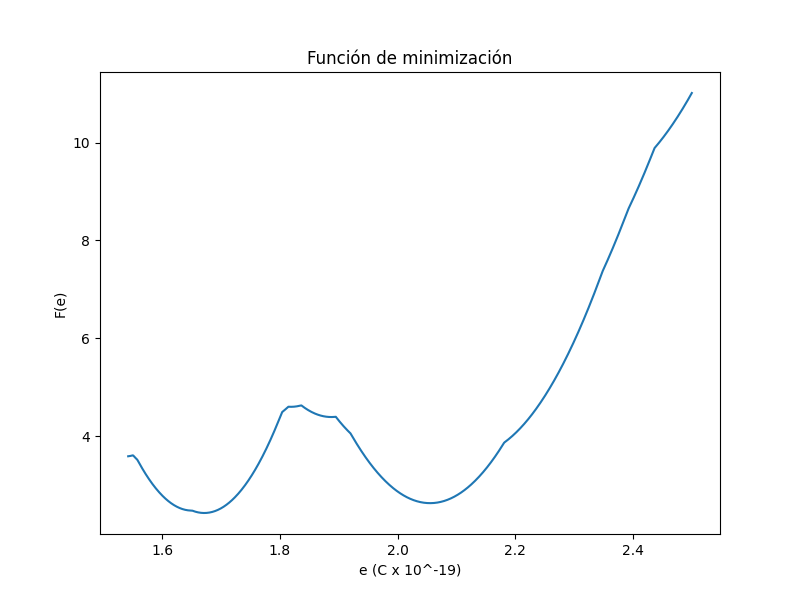
\includegraphics[width=0.7\columnwidth]{img/F_vs_e.png}
        \caption{Función de dispersión $F(\hat{e})$ evaluada para diferentes valores de prueba.}
        \label{fig:funcion-perdidas-carga-elec}
    \end{figure}

Tras la optimización y búsqueda del mínimo global de la función de pérdidas, se alcanzó un valor preeliminar para la carga fundamental de $\hat{e} \approx 1.67 \cdot 10^{-19}$ C. 

Aunque este podría considerarse el valor resultante, el cálculo directo mediante la minimización previa incluye un redondeo interno en el cociente que no satisface estrictamente la hipótesis de cuantización en cada gota individual, hipótesis la cual representa el pilar fundamental del estudio. Para asegurar que cumplimos con la física supuesta, se forzó la discretización: se dividió cada carga total medida $q_i$ entre el valor estimado de $\hat{e}$, extrayendo el número entero de portadores ($n_i$). A continuación, se recalculó la carga elemental específica aportada por cada gota ($e_i = q_i / n_i$). Finalmente, mediante una media ponderada en función de sus incertidumbres relativas, se determinó el valor global de la carga elemental y se contrastó con el referencial.

Los valores de carga elemental deducidos para cada microgota aislada se recogen en la siguiente tabla:

\begin{table}[hbt!]
\centering
\begin{tabular}{lc}
\hline
n & $e$ ($10^{-19}$ C) \\
\hline
gota 1  & $1.79 \pm 0.05$ \\
gota 2  & $1.89 \pm 0.05$ \\
gota 3  & $1.61 \pm 0.03$ \\
gota 4  & $1.60 \pm 0.03$ \\
gota 5  & $1.50 \pm 0.03$ \\
gota 6  & $2.11 \pm 0.10$ \\
gota 7  & $1.82 \pm 0.03$ \\
gota 8  & $1.93 \pm 0.10$ \\
gota 9  & $2.31 \pm 0.10$ \\
gota 10 & $2.48 \pm 0.10$ \\
gota 11 & $1.59 \pm 0.03$ \\
gota 12 & $1.58 \pm 0.03$ \\
gota 13 & $1.64 \pm 0.10$ \\
gota 14 & $1.76 \pm 0.05$ \\
gota 15 & $1.71 \pm 0.02$ \\
gota 16 & $1.73 \pm 0.10$ \\
\hline
\end{tabular}
\vspace{0.1cm}
\caption{Valor estimado de la carga elemental ($e$) para cada gota}
\label{tab:carga_elemental_gotas}
\end{table}

Agrupando todos los eventos medidos y aplicando la media ponderada estipulada por la expresión teórica:

\begin{equation}
e \pm \Delta e = \frac{\sum w_i e_i}{\sum w_i} \pm \frac{1}{\sqrt{\sum w_i}} \quad \text{con} \quad w_i = \left( \frac{1}{\Delta e_i} \right)^2
\end{equation}

Se obtuvo el siguiente resultado empírico definitivo para la carga del electrón:
\vspace{0.2cm}
\begin{equation*}
\boxed{e = (1.672 \pm 0.009) \times 10^{-19} \text{ C}}
\end{equation*}

\section{Conclusiones}

Tras el análisis de los datos experimentales, se ha obtenido un valor para la carga elemental de $e = (1.672 \pm 0.009) \times 10^{-19}$ C. Al comparar este resultado con el \textbf{valor referencial} de $1.602 \times 10^{-19}$ C, se observa una desviación del 4.3\%. Dado que la incertidumbre estadística obtenida es muy pequeña, esta diferencia sugiere la presencia de errores sistemáticos en el montaje, como posibles imprecisiones en la medición de la distancia entre las placas del condensador ($d = 3$ mm) o variaciones locales en la viscosidad del aire debido al calentamiento producido por la iluminación del microscopio.

El experimento ha permitido verificar de forma clara la cuantización de la carga eléctrica. La función de dispersión $F(\hat{e})$ mostró mínimos muy definidos, lo que confirma que las cargas medidas en las gotas no siguen una distribución continua, sino que son múltiplos enteros de una unidad fundamental. Asimismo, se ha comprobado que la corrección de Cunningham a la ley de Stokes es indispensable en este rango de medidas; sin ella, el cálculo de los radios microscópicos y de la carga total carecería de sentido físico al no tener en cuenta el camino libre medio del aire.

En resumen, tanto el método dinámico como el de suspensión han resultado ser consistentes y adecuados para los objetivos de la práctica. A pesar de las dificultades experimentales inherentes al seguimiento óptico de las microgotas, los resultados obtenidos validan con éxito la hipótesis de Millikan y permiten una determinación de la carga del electrón con un grado de precisión notable.
\appendix
\section{Cálculo de Errores}

Para dotar de rigor estadístico a los valores presentados, se ha realizado una propagación de incertidumbres considerando los límites de precisión propios del instrumental descrito en el guion de la práctica.

\subsection*{1. Incertidumbres directas del instrumental}

Se asumen los siguientes márgenes de error sistemático aportados por los aparatos de medida:
\begin{itemize}
    \item Distancia entre las placas del condensador: $\delta d = \pm 0.1$ mm.
    \item Distancia transitada en la escala del ocular: $\delta s = \pm 50$ $\mu$m.
    \item Error en la lectura de la tensión aplicada: $\delta U = \pm 0.5\%$ del valor nominal medido.
    \item Error instrumental en el cronometraje de los intervalos: $\delta t_{inst} = \pm 100$ ms.
\end{itemize}

\subsection*{2. Incertidumbre en los tiempos de tránsito}
Para minimizar la fluctuación estadística debida a la manipulación del cronómetro, se tomaron varias medidas ($n$) del tiempo de ascenso y descenso de cada gota. El error final asignado a cada tiempo ($t_i$) se ha tomado como el valor máximo entre la resolución instrumental y la desviación estándar de las medidas:
\vspace{0.2cm}
\begin{equation*}
    \delta t = \max \left( 0.1 \text{ s} \; , \; \sqrt{\frac{1}{n-1}\sum_{j=1}^{n} (t_{j} - \bar{t})^2} \right)
\end{equation*}
\vspace{0.2cm}

\subsection*{3. Incertidumbre en las velocidades}
Conociendo la distancia recorrida ($s$), el tiempo ($t_i$) y el aumento de la lente ($V=2$), la velocidad cinemática se determina como $v_i = s / (V \cdot t_i)$. Su incertidumbre propagada relativa corresponde a la suma en cuadratura de sus variables dependientes:
\vspace{0.2cm}
\begin{equation*}
    \frac{\delta v_i}{v_i} = \sqrt{\left(\frac{\delta s}{s}\right)^2 + \left(\frac{\delta t_i}{t_i}\right)^2}
\end{equation*}
\vspace{0.2cm}

\subsection*{4. Incertidumbre en los parámetros corregidos ($r$ y $q$)}

Dado que tanto el radio como la carga final dependen de múltiples variables indirectas ($v_1, v_2, U, d$) afectadas a su vez por la corrección de Stokes, la propagación analítica exacta se deduce empleando la suma en cuadratura de las derivadas parciales respecto a cada variable medida:
\vspace{0.2cm}
\begin{equation*}
    \delta q = \sqrt{ \sum_{x \in \{U, v_1, v_2, d\}} \left( \frac{\partial q}{\partial x} \delta x \right)^2 }
\end{equation*}
\vspace{0.2cm}

Este mismo procedimiento de derivación parcial se aplicó de manera análoga para la obtención del error empírico del radio corregido ($\delta r$).

\subsection*{5. Incertidumbre de la carga elemental por gota ($e_i$) y media ponderada}

Al dividir la carga corregida de una gota entre el número de electrones que alberga, obtenemos su aportación individual al valor de $e$. Dado que el número de cargas ($n_i$) es un entero discreto exacto sin incertidumbre inherente, la propagación es directa:
\vspace{0.2cm}
\begin{equation*}
    \delta e_i = \frac{\delta q_i}{n_i}
\end{equation*}
\vspace{0.2cm}

El valor final, representativo de todas las gotas analizadas, requiere dar mayor relevancia estadística a las mediciones con menor margen de error. Esto se consigue empleando el factor de peso $w_i = 1 / (\delta e_i)^2$. El error de esta media ponderada queda definido por:
\vspace{0.2cm}
\begin{equation*}
    \delta e = \frac{1}{\sqrt{\sum w_i}}
\end{equation*}
\vspace{0.2cm}

\end{document}